\begin{abstract}
Incremental matrix maintenance reuses previous products, but output
correctness alone does not quantify the fresh computation behind an
accepted update. We derive work-sensitive acceptance bounds for a stateful
finite-field interface: a homogeneous bilinear program is selected before
fresh update factors arrive, and its complete candidate is fixed before
random verification. The processor may retain arbitrary previously paid
state. For uniform factors, conditioning on matrix rank yields an
output-span agreement profile that improves the corresponding range-size
estimate at every positive gate budget below the number of entries in one
factor.
A resource recursion composes the profiles under adaptive pathwise budgets,
including incorrectly accepted intermediate states. Conditional linear
escape extends the threshold guarantee to nonuniform factors. Balanced
checking minimizes the homogeneous certificates, and an exact allocator
minimizes the heterogeneous threshold certificate under equal check costs.
A six-product $2\times2$ Strassen construction attains the single-round
threshold bound. Exact-field experiments include candidate materialization
and verification: at matrix dimension 4096, update width eight, and field
size 65521, reuse reduces graphics-processor latency from $161.93$ to
$83.16$\,ms, a paired $1.95\times$ speedup. Randomized categorical views
connect report encoding, statistical accuracy, and fresh-work guarantees.
At field size 17, parameter-aware checking allocation saves $10.4\%$ of checks
relative to fixed-prefix round robin and $1.4\%$ of measured service and
planning time over twenty processor sessions.
\end{abstract}

\section{Introduction}\label{sec:introduction}
Matrix products arise in analytical views, matrix chains, and feature
transformations that must remain current as records change. Incremental
view maintenance exploits previous results rather than recomputing them;
higher-order maintenance, linear-algebra programs, and factorized analytics
provide established techniques for doing so\cite{dbtoaster,Linview2014,fivm}.
Let $n$ be the matrix dimension, $r$ the update width with $n\ge r\ge2$,
and $\F_q$ the finite field with $q$ elements. For
$A,B\in\F_q^{n\times n}$ with $B$ fixed and invertible, the maintained
product is $C=AB$. Fresh factors $U,V\in\F_q^{n\times r}$ specify
$A'=A+UV^\top$, giving the standard update identity
\[
 C'=A'B=C+U(V^\top B).
\]
The identity reduces arithmetic through reuse. Our question is how that
reuse interacts with verification when another processor supplies the
updated product.


\begin{figure*}[!t]
  \centering
  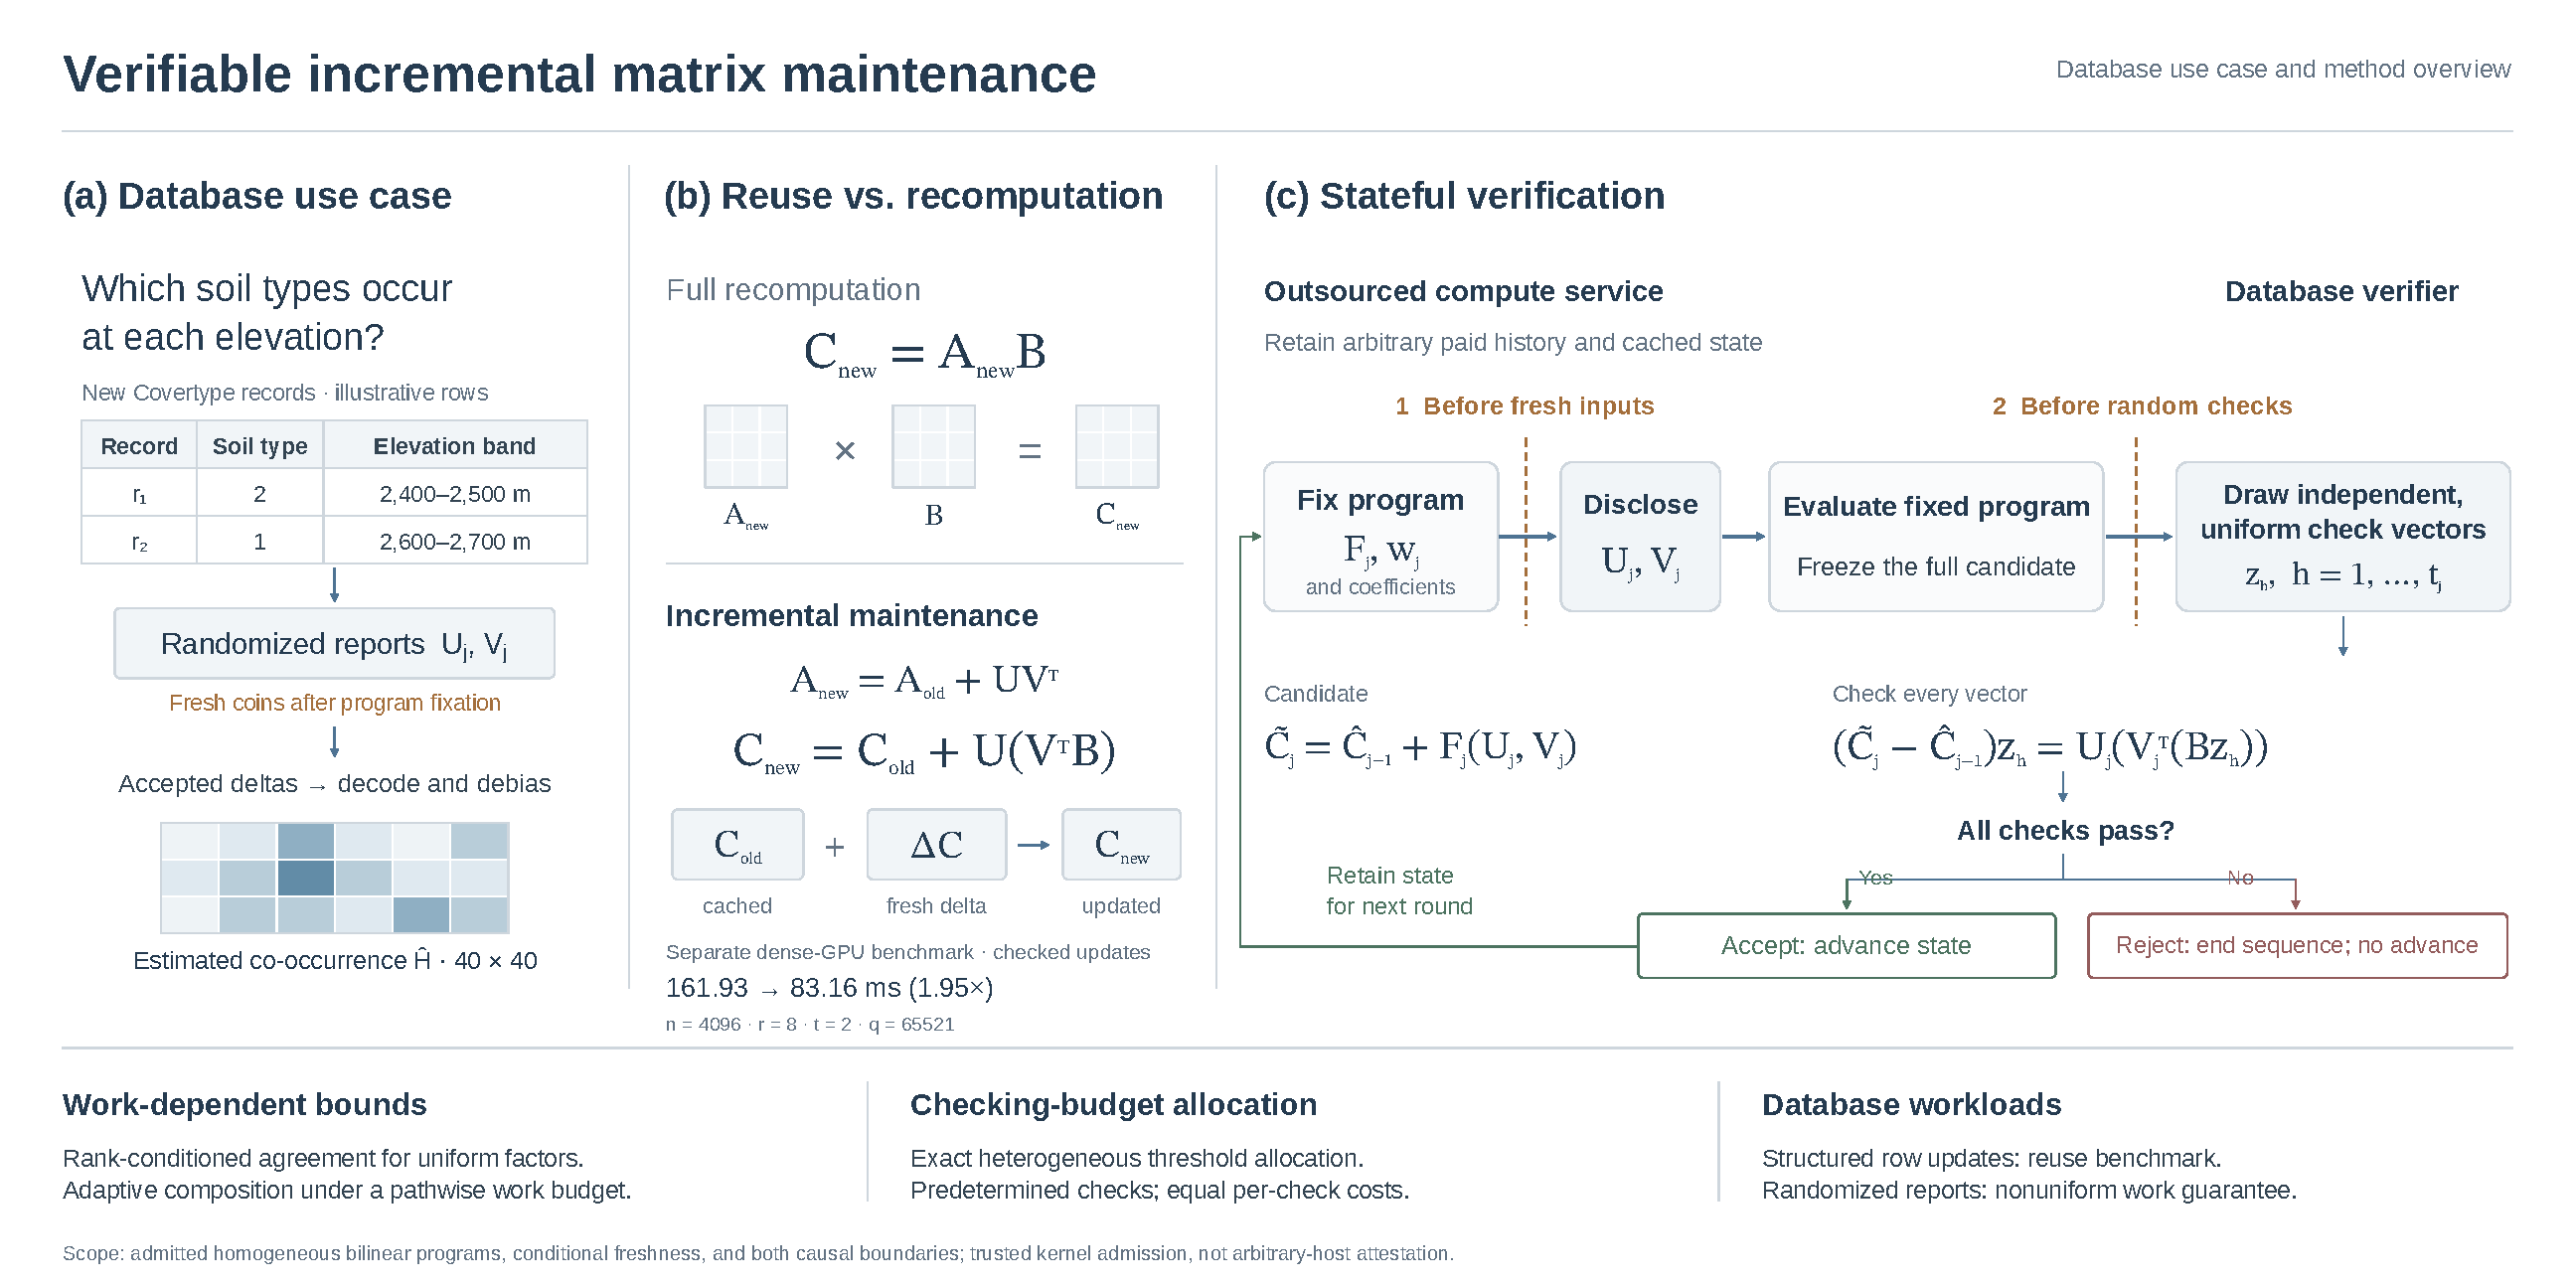
\includegraphics[width=\textwidth]{figures/ICDE_figure_simplified.pdf}
  \caption{Database use case and verifiable incremental matrix maintenance.
  (a) Covertype records yield randomized soil-type and elevation-band reports;
  the schematic co-occurrence heatmap represents a decoded, debiased estimate,
  not the retained modular state. (b) A cached product is updated using
  $U(V^\top B)$ instead of full recomputation; the dense-GPU timing is a
  separate workload. (c) The admitted bilinear program and gate count are
  fixed before fresh factors arrive, and the complete candidate is fixed
  before independent random checks. Acceptance advances the reference;
  rejection ends the prescribed sequence.}
  \label{fig:fresh-flow}
\end{figure*}

Figure~\ref{fig:fresh-flow} illustrates the motivating analytical view and
the causal protocol. In the Covertype application, 40 soil categories and
40 elevation bins of width 100\,m over $[0,4000)$ define the
soil--elevation domain. Fresh randomized reports update a retained
finite-field matrix; accepted report increments are decoded and debiased
into a separate noisy co-occurrence estimate. The heatmap is schematic,
not measured data. The latency annotation concerns a distinct
$n=4096$, $r=8$, $t=2$, $q=65521$ dense-GPU experiment, rather than
the Covertype view. The two causal boundaries allow reuse of arbitrary
paid historical state, while the fresh-work certificate remains
conditional on the admitted homogeneous bilinear program class and
trusted kernel admission, not physical-work attestation.

Random projections efficiently check a fixed candidate\cite{freivalds},
but a correctness check does not by itself measure the computation used to
produce it. A processor can retain earlier inputs, products, and auxiliary
state, then adapt its computation to the observed history. Relating
acceptance to fresh work therefore requires a bound that remains valid
after each such history and composes across adaptively chosen updates.
Incorrectly accepted intermediate products make this a stateful problem:
the next check may start from a reference that is already wrong.

We study a homogeneous bilinear interface in which a program with $w$
gates is fixed before the current factors arrive. Each gate multiplies
one linear form in $U$ by one in $V$; $w$ counts these products across all
suppliers. Historical state may select the program, while the complete
candidate precedes the verifier's independent random vectors.
Section~\ref{sec:fresh-updates} specifies the interface and its cost
accounting. The prototype realizes it through trusted kernel admission.

The key insight is to retain the rank information in the agreement
analysis. For independent uniform factors conditional on a fixed history,
conditioning on $U$ of rank $s$ makes $UV^\top B$ uniform on an
$ns$-dimensional matrix subspace. The program's outputs lie in the span
of its coefficient matrices, whose dimension is at most $w$. Bounding
their intersection within each rank stratum and then averaging yields an
explicit agreement profile. It is strictly smaller than the capped
range-size estimate for every integer $0<w<nr$. A backward resource
recursion then converts these one-round profiles into a bound for a
prescribed sequence under a work budget that holds on every execution
path. This separates the effect of retained information from computation
on the newly disclosed factors.

Our contributions connect this analysis to checking decisions and
maintained analytical state:
\begin{itemize}
\item \textbf{Work-sensitive, stateful bounds.} We derive the rank-conditioned
agreement profile and its adaptive composition, including incorrect
intermediate references (Lemma~\ref{ext:lem-output-span} and
Theorem~\ref{ext:thm-profile-dp}). Conditional linear escape supplies
threshold bounds for nonuniform factors.
\item \textbf{Certificate-optimal checking.} We prove balanced allocation
optimal for the homogeneous certificates and give an exact allocator for
the heterogeneous threshold certificate under equal checking costs
(Theorems~\ref{ext:thm-balanced} and~\ref{ext:thm-heterogeneous}).
A six-product construction attains the single-round threshold bound
(Theorem~\ref{ext:thm-sharpness}).
\item \textbf{End-to-end evaluation and a nonuniform application.} Exact-field
implementations measure reuse together with materialization and checks.
Fresh randomized attribute reports instantiate the nonuniform assumptions
and expose the relationship between encoding accuracy, work-target
feasibility, and integrity-driven checking budgets
(Sections~\ref{sec:execution}--\ref{sec:evaluation}).
\end{itemize}

\section{Related Work}\label{sec:related}
\paragraph{Incremental analytics}
DBToaster develops higher-order maintenance, LINVIEW treats linear-algebra
programs, and F-IVM combines factorization with ring-based analytics
\cite{dbtoaster,Linview2014,fivm}. These techniques optimize maintained
values under updates. Our analysis adds a work-sensitive acceptance bound
for a processor that retains state, while using the established product
update as its application interface.

\paragraph{Verification and useful work}
Freivalds' random projections verify dense matrix products using quadratic
field-operation cost per check\cite{freivalds}. Pantry supports verifiable
computation over persistent storage\cite{Pantry2013}, while Dumas and Zucca
amortize public matrix-vector verification through preprocessing
\cite{DumasZucca2017}. These verification mechanisms concern output
correctness; our certificates additionally relate acceptance to a fresh
bilinear-work budget. Komargodski and Weinstein study useful-work proofs
for arbitrary matrix multiplication, with their strongest security claim
based on correlated low-rank linear systems\cite{kwesa}. Our guarantees
are information-theoretic within the stated online program class.
Alman's lookup-table algorithms distinguish finite-field bit complexity
from arithmetic-gate counts\cite{alman_lookup}; our work accounting uses
the latter, with other execution costs measured separately.

\paragraph{Bilinear agreement}
Tensor rank underlies exact bilinear computation\cite{algebraic,strassen}.
Cohen and Moshkovitz relate analytic, geometric, and slice rank
\cite{cohen2022structure}, and the geometric rank of rectangular
multiplication is known\cite{kopparty2023geometric}. Using classical
finite-field matrix-rank counts\cite{LaksovThorup1994}, our output-span
argument conditions on the input rank before averaging the agreement
bound. Section~\ref{ext:sec-profile} compares the resulting profile
with the rank-based and range-size bounds. The six-product witness is
related to defective products in probabilistic tensor algorithms
\cite{KarppaKaski2019}; the seven-product threshold also follows from the
support-rank result of Bl\"aser et al.\cite{BlaserChristandlZuiddam2017}.

\paragraph{Allocation and application mechanisms}
Our heterogeneous allocator specializes ordered-sum thresholds
\cite{OgryczakTamir2003} and separable concave resource allocation
\cite{FedergruenGroenevelt1986} to the acceptance certificate. The categorical
application uses established symmetric and optimized unary encodings
\cite{wang2017local}: their report distributions determine the conditional
escape parameters, connecting encoding accuracy to work-target feasibility.
Output integrity imposes a separate checking constraint. Exact word-size
field arithmetic follows the implementation approach of FFLAS-FFPACK
\cite{dumas2008fflas}.
